\documentclass[sutton_barto_notes.tex]{subfiles}
\begin{document}

\newpage
\textbf{Part II: Approximate Solution Methods}
In the second part, we are dealing with arbitrarily large state spaces; in these cases, it is hard to find $\pi_*$ or $v_*, q_*$.
Our goal instead is to find a good approximate solution using limited computational resources.

The problem with large state spaces is threefold: memory, time and data.
In many of our target tasks, almost every state encountered will never have been seen before. The solution is \textit{generalization}.
How can experience with a limited subset of the state space be usefully generalized to produce a good approximation over a much larger subset?

To some extent, we need only combine RL methods with existing  generalization methods. One of frequent use is \textit{function approximation}, which takes examples from a desired function (e.g. a value function) and attempts to generalize from them to construct an approximation of the entire function.

Function approximation is an instance of supervised learning.

RL with function approximation involves a number of new issues (usually not in SL), such as nonstationarity, bootstrapping, and delayed targets.

Chap 9 (prediction): on-policy training, policy is given and only its value function is approximated

Chap 10 (control): an approximation to the optimal policy is found

Chap 11: off-policy learning with function approximation

Chap 12: \textit{eligibility traces}, which dramatically improves the computational properties of multi-step RL methods in many cases.

Chap 13 (control): \textit{policy-gradient}, a different approach to control, which approximates the optimal policy directly and need never form an approximate value function.

\newpage
\section{On-policy Prediction with Approximation}

We start consider using function approximation in estimating the state-value function from on-policy data, which approximates $v_\pi$ from experience generated using a known policy $\pi$.

The approximate value function is represented as a parameterized functional form with weight vector $\bm{w} \in \R^d$, instead of a table.
We write $\hat{v}(s,\bm{w}) \approx v_\pi(s)$ for the approximate value of state $s$ given weight vector $\bm{w}$.

For example,
\begin{itemize}
\item $\hat{v}$ = linear function in features of the state, $\bm{w}$ = vector of feature weights
\item $\hat{v}$ = function computed by a multi-layer ANN, $\bm{w}$ = vector of connection weights in all the layers
\item $\hat{v}$ = function computed by a decision tree, $\bm{w}$ = all the numbers defining the split points and leaf values of the tree
\end{itemize}

Typically, the number of weights is much less than the number of states ($d <<|S|$), and one weight takes care of many states.

Extending RL to function approximation also makes it applicable to partially observable problems (in which the full state is not available to the agent).

All theoretical results for methods using function approximation apply equally well to cases of partial observability.

Function approximation cannot augment the state representation with memories of past observations.

\subsection{Value-function Approximation}

\begin{definition}
\textbf{individual update notation}: $s \rightarrow u$ (the book uses $|->$, where $s$ is the state updated and $u$ is the update target. The estimated value for $s$ should be more like $u$.
\end{definition}

\begin{itemize}
\item MC: $S_t \rightarrow G_t$
\item TD(0): $S_t \rightarrow R_{t+1} + \gamma \hat{v}(S_{t+1},\bm{w}_t)$
\item n-step TD: $S_t \rightarrow G_{t:t+n}$
\item DP: $s \rightarrow \E_\pi [R_{t+1} + \gamma \hat{v}(S_{t+1}, \bm{w}_t) | S_t = s]$
\end{itemize}

We want to extend a one-to-one mapping to one-to-many mapping, i.e., updating $s$ will also update many other states.

Supervised learning methods learn to mimic input-output examples, and when the outputs are numbers, like $u$, the process is often called \textit{function approximation}.
We use these methods for value prediction simply by passing to them the $s \rightarrow u$ of each update as a training example.

In principle, we can use any method for supervised learning from examples, including ANN, decision trees, and various kinds of multivariate regression.
However, in RL, we require the methods are able to handle nonstationarity cases as RL agents need to do online learning (interact with the environment to obtain data).

\subsection{The Prediction Objective ($\overline{VE}$)}

By assumption we have far more states than weights, so making one state's estimate more accurate invariably(always) means making others' less accurate. We need to find which states we care most about. Therefore, we introduced the state distribution $\mu(s)$:
\begin{definition}
\textbf{state distribution $\mu(s)$}: $\mu \geq 0$, $\sum_s \mu(s) = 1$, representing how much we care about the error (square distance between approx value $\hat{v}(s,\bm{w})$ and true value $v_\pi(s)$) in each state $s$.
\end{definition}

Since we are doing on-policy policy evaluation, the $\mu$ is from policy $\pi$. We can also design $\mu$, then it becomes off-policy prediction.

\begin{definition}
\textbf{Mean Squared Value Error ($\overline{VE}$)}: a natural objective function,
$$\overline{VE}(\bm{w}) \doteq \sum_{s\in S} \underbrace{\mu(s)}_{\text{weight}} \underbrace{[v_\pi(s) - \hat{v}(s,\bm{w})]^2}_{\text{error}}$$
\end{definition}

Often $\mu(s)$ is chosen to be the fraction of time spent in $s$. Under on-policy training, this is called \textit{on-policy distribution}. In continuing tasks, the on-policy distribution is the stationary distribution under $\pi$. The book talks about the episodic tasks (not including here).

!! NOTE that the RL community is not sure if $\overline{VE}$ is the right performance objective for RL. But this is the best we can find so far. Adam White: VE might not be the best because we are only approximating the exact true values. Instead, we can use Average reward + Policy Gradient methods for control.

\subsection{Stochastic-gradient and Semi-gradient Methods}

In GD, the weight vector is a column vector with a fixed number of real valued components, $\bm{w} \doteq (w_1, w_2, ..., w_d)^T $, and the approximate value function $\hat{v}(s,\bm{w})$ is a differentiable function of $\bm{w}$ for all $s \in S$. However, no $\bm{w}$ can gets all the states in real world.

\paragraph{GD vs SGD} In both GD and SGD, we update a set of parameters in an iterative manner to minimize an error function.
\begin{itemize}
\item GD: we run through ALL the samples to do a single update for a parameter in a particular iteration (which is not feasible)
\item SGD: we run through ONLY ONE or a SUBSET of samples to do the update. If we use a SUBSET, it is called Minibatch Stochastic Gradient Descent.
\end{itemize}

The solution to $\bm{w}$ is SGD: we minimize error on the \textit{observed samples}. The weight vector of SGD is:
$$ \bm{w}_{t+1} \doteq \bm{w} - \frac{1}{2}\alpha \nabla [v_\pi(S_t) - \hat{v}(S_t, \bm{w}_t)]^2$$
$$ \bm{w}_{t+1} = \bm{w} + \alpha[v_\pi(S_t) - \hat{v}(S_t, \bm{w}_t)]\nabla \hat{v}(S_t, \bm{w}_t) $$

Now we consider when we do not have the exact true value $v_\pi(S_t)$, but an approximate value $U_t$. Then
$$ \bm{w}_{t+1} = \bm{w} + \alpha[U_t - \hat{v}(S_t, \bm{w}_t)]\nabla \hat{v}(S_t, \bm{w}_t) $$

If $U_t$ is an \textit{unbiased} estimate ($\E[U_t|S_t=s]=v_\pi(s)$), then $\bm{w}_t$ is guaranteed to converge to a local optimum under the usual stochastic approximation conditions (chap2). For example, Monte Carlo target $U_t\doteq G_t$ is an unbiased estimate of $v_\pi(S_t)$.

\begin{tcolorbox}[width=1.1\textwidth,title={Gradient Monte Carlo for Estimating $\hat{v}\approx v_\pi$}]
Input: $\pi$ to be evaluated, a differentiable function $\hat{v}:S\times\R^d \rightarrow \R$

Parameter: $\alpha > 0$

Init the value-function weights $\bm{w} \in \R^d$ arbitrarily

Loop forever (for each episode):

$\quad$Generate an episode $S_0, A_0, R_1, S_1, A_1, ..., R_T, S_T$ using $\pi$

$\quad$Loop for each step of episode, $t = 0,1,...,T-1$:

$\quad$Take action $A$; observe resultant reward, $R$, and state, $S'$

$\quad\quad$ $\bm{w} \leftarrow \bm{w} + \alpha [ G_t - \hat{v}(S_t, \bm{w})]\nabla \hat{v}(S_t, \bm{w})$
\end{tcolorbox}

On the other hand, Bootstrapping targets, such as $n$-step returns $G_{t:t+n}$ or the DP target, all depend on the current value of the weight vector $\bm{w}_t$, which implies that they will be biased. These are not the true gradient-descent methods, but $semi$-gradient methods.

Although semi-gradient (bootstrapping) methods do not converge as robustly as true gradient methods, they offer important advantages: (1) enable much faster learning; (2) enable learning to be continual and online; (3) provides computational advantages. A typical semi-gradient method is semi-gradient TD(0), which uses $U_t \doteq R_{t+1} + \gamma \hat{v}(S_t, \bm{w})$

\begin{tcolorbox}[width=1.1\textwidth,title={Semi-gradient TD(0) for Estimating $\hat{v}\approx v_\pi$}]
Input: $\pi$ to be evaluated, a differentiable function $\hat{v}:S\times\R^d \rightarrow \R$ where $\hat{v}(terminal,\dot)=0$

Parameter: $\alpha > 0$

Init the value-function weights $\bm{w} \in \R^d$ arbitrarily

Loop for each episode:

$\quad$Init $S$

$\quad$Loop for each step of episode:

$\quad\quad$Choose $A$~$\pi(\dot | S)$

$\quad\quad$Take action $A$; observe reward, $R$, and state, $S'$

$\quad\quad$ $\bm{w} \leftarrow \bm{w} + \alpha [ R + \gamma \hat{v}(S_t, \bm{w}) - \hat{v}(S,\bm{w})]\nabla \hat{v}(S_t, \bm{w})$

$\quad\quad S \leftarrow S'$

$\quad$until $S$ is terminal
\end{tcolorbox}

The target $U_t$ in semi-gradient methods is biased, so the $\bm{w}$ may not converge to a local optimum.



\paragraph{state aggregation} a simple form of generalizing function approximation in which states are grouped together, with one estimated value for each group.



\subsection{Linear Methods}

One of the most important special cases of function approximation is that, $\hat{v}(\dot, \bm{w})$ is a linear function of the weight vector $\bm{w}$. Corresponding to every state $s$, there is a real-valued vector $\bm{x}(s)\doteq (x_1(s),x_2(s),...,x_d(s))^T$, with the same number of components as $\bm{w}$.

Linear methods approximate the state-value function by the inner product between $\bm{w}$ and $\bm{x}(s)$:
$$\hat{v}(s,\bm{w}) \doteq \bm{w}^T\bm{x}(s)\doteq \sum_{i=1}^d w_i x_i(s) $$

The vector $\bm{x}(s)$ is a \textit{feature vector} representing state $s$. Each component $x_i(s)$ is a \textit{feature}.

The gradient of the approximation value function w.r.t $\bm{w}$ is then $\nabla\hat{v}(s,\bm{w})=\bm{x}(s)$.
Thus, we can simplify the general SGD update to
$$\bm{w}_{t+1} = \bm{w} + \alpha[U_t - \hat{v}(S_t, \bm{w}_t)]\bm{x}(s)$$

\paragraph{Understand the fixed point of linear TD learning}

Let us start with TD update with linear function approximation on the first line, recall the value of a state $\hat{v}(s,\bm{w}) \doteq \bm{w}^T\bm{x}(s)$
\begin{align*}
\bm{w}_{t+1} &\doteq \bm{w} + \alpha[R_{t+1} + \gamma\hat{v}(S_{t+1},\bm{w}_t) - \hat{v}(S_t, \bm{w}_t)]\bm{x}(S_t) \\
&= \bm{w} + \alpha[R_{t+1} + \gamma\hat{v}(S_{t+1},\bm{w}_t) - \hat{v}(S_t, \bm{w}_t)]\bm{x}_t \quad \text{simplify notation}\\
&= \bm{w} + \alpha[R_{t+1} + \gamma\bm{w}_t^T\bm{x}_{t+1} - \bm{w}_t^T\bm{x}_t]\bm{x}_t \quad \text{due to }\hat{v}(s,\bm{w}) \doteq \bm{w}^T\bm{x}(s)\\
&= \bm{w} + \alpha[\underbrace{R_{t+1}\bm{x}_t}_{\bm{b}} - \underbrace{\bm{x}_t(\bm{x}_t - \gamma\bm{x}_{t+1})^T}_{\bm{A}}\bm{w}_t] \quad\text{transpose doesn't change scalar}\\
\end{align*}
The TD update can be rewritten as the expected update + a noise term, so it is largely dominated by the behavior of the expected update.
\begin{align*}
\E[\Delta \bm{w}_t] &= \alpha(\bm{b} - \bm{A}\bm{w}_t) \\
\bm{b} &= \E[R_{t+1}\bm{x}_t] \\
\bm{A} &= \E[\bm{x}_t(\bm{x}_t - \gamma\bm{x}_{t+1})^T] \quad \text{expct. over features}
\end{align*}

\begin{definition}
\textbf{TD Fixed Point $\bm{w}_{TD}$}, the weight is converged when the expected TD update = 0. TD fixed point is the solution to the semi-gradient TD(0).
$$\E[\Delta \bm{w}_{TD}] = \alpha(\bm{b} - \bm{A}\bm{w}_{TD}) = 0$$
\end{definition}
When $A$ is invertible, we can rewrite $\bm{w}_{TD} = \bm{A}^{-1}\bm{b}$. We say $\bm{w}_{TD}$ is a solution to this linear system; the solution is called TD fixed point.

$\bm{w}_{TD}$ minimizes an objective that is based on this $\bm{A}$ and $\bm{b}$. This objective extends the connection between TD and Bellman equations to the function approximation setting.

Recall in the tabular setting, TD is described as a sample based method for solving the Bellman equation. Linear TD similarly approximates the solution to the Bellman equation, minimizing what is called the projected Bellman error.

\paragraph{Describe a theoretical guarantee on the mean squared value error at the TD fixed point}

We want to understand the relationship between the solution found by TD and the minimum value error solution.
$$\overline{VE}(\bm{w}_{TD}) \leq \frac{1}{1-\gamma}min_{\bm{w}}\overline{VE}(\bm{w})$$
The difference between these two errors depends on $\gamma$ and the quality of features.

Why isn't the TD fixed point error equal to the minimum value error solution? This is because bootstrapping under function approximation. If our function approximator is good, then our estimate of the next state will be accurate.

\begin{tcolorbox}[width=1.1\textwidth,title={n-step semi-gradient TD for estimating $\hat{v}\approx v_\pi$}]
Input: $\pi$ to be evaluated, a differentiable function $\hat{v}:S\times\R^d \rightarrow \R$ where $\hat{v}(terminal,\dot)=0$

Parameter: $\alpha > 0$, $n > 0$

Init the value-function weights $\bm{w} \in \R^d$ arbitrarily

All store and access operations ($S_t$ and $R_t$) can their index mod $n+1$

Loop for each episode:

$\quad$Init and store $S_0 \neq$ terminal

$\quad T \leftarrow \inf$

$\quad$Loop for t = 0,1,2,...:

$\quad\quad$If $t<T$,then:

$\quad\quad\quad$Take an action according to $\pi(\cdot|S_t)$

$\quad\quad\quad$Observe and store $R_{t+1}$ and $S_{t+1}$

$\quad\quad\quad$If $S_{t+1}$ is terminal, then $T \leftarrow t+1$

$\quad\quad\tau \leftarrow t-n+1$ ($\tau$ is the time whose state's estimate is being updated)

$\quad\quad$If $\tau \geq 0$:

$\quad\quad\quad G \leftarrow \sum_{i=\tau + 1}^{min(\tau+n,T)} \gamma^{i-\tau-1}R_i$

$\quad\quad\quad$If $\tau + n < T$, then: $G\leftarrow G+\gamma^n \hat{v} (S_{\tau + n}, \bm{w})$

$\quad\quad\quad \bm{w} \leftarrow \bm{w} + \alpha [G - \hat{v}(S_{\tau},\bm{w})]\nabla \hat{v}(S_{\tau},\bm{w})$

$\quad$until $\tau = T-1$
\end{tcolorbox}

\subsection{Feature Construction for Linear Methods}

Choosing features appropriate to the task is an important way of adding \textit{prior domain knowledge} to reinforcement learning systems.

Linear methods,
\begin{itemize}
\item pro: guarantee convergence, data efficient, computation efficient
\item con: does not consider interactions between features
\end{itemize}

\subsubsection{Polynomials}
\subsubsection{Fourier Basis}
\subsubsection{Coarse Coding}

The features used to construct value estimates, are one of the most important parts of a RL agent.

Recall linear value function approximation $v_\pi(s) \approx \hat{v}(s,\bm{w}) = \bm{w}^T\bm{x}(s)$. Recall that a tabular representation can be expressed as a binary (0 or 1) feature vector. Each state is associated with a different feature. Agent-presented state is 1, all other features are 0. The tabular case is a special case of linear function approximation, where the feature vector is an indicator/one-hot encoding of the state.

This becomes a problem when the feature space is large. Recall that we can use state aggregation to associate nearby states with the same features.

From state aggregation to coarse coding: although state aggregation can have arbitrary shapes, but it does not allow overlapping. We can remove this restriction, and we have coarse coding. Therefore, coarse coding is a generalization of state aggregation.

\begin{definition}
\textbf{binary feature}: 1-0 valued feature, 1 for present, 0 for absent.
\end{definition}
\begin{definition}
\textbf{coarse coding}: representing a state with binary features that overlap.
\end{definition}

\begin{figure}[h!]
  \centering
  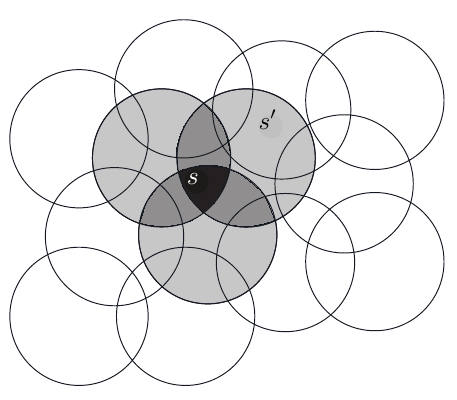
\includegraphics[width=0.5\linewidth]{c9-coarse-coding.png}
  \caption{Coarse coding. Generalization from $s$ to $s'$ depend on the number of their features whose receptive fields overlap}
  \label{fig:coarse-coding}
\end{figure}

Changing the shapes and sizes of features impacts generalization and discrimination, and so affects the speed of learning and the value functions we can represent.

Coarse coding parameters affect discrimination and generalization, which in turn affect learning accuracy.

\begin{figure}[h!]
  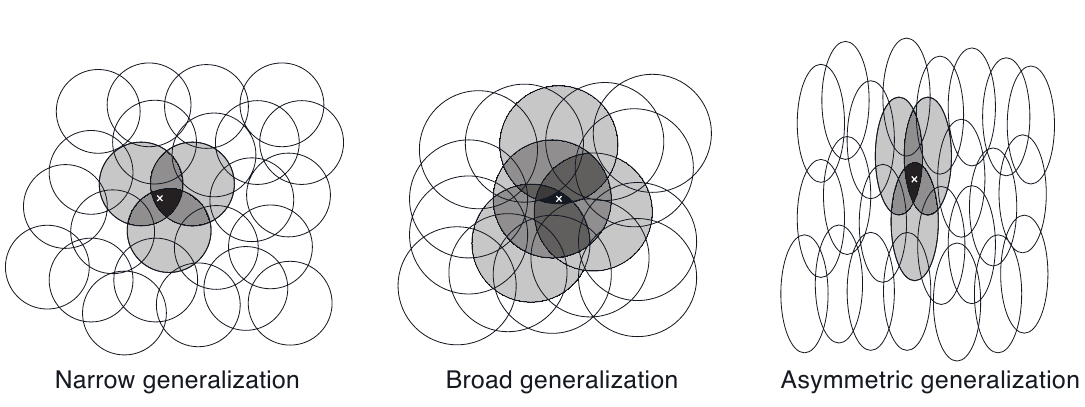
\includegraphics[width=1\linewidth]{c9-coarse-coding-2.png}
  \caption{Generalization in linear function approximation methods is determined by the sizes and shapes of the features' receptive fields. All three of these cases have roughly the same number and density of features.}
  \label{fig:coarse-coding-2}
\end{figure}

\clearpage % needed when there are float figures
\newpage
\subsubsection{Tile Coding}

\begin{definition}
\textbf{Tile coding}, a form of coarse coding for multi-dimensional continuous spaces that is flexible and computationally efficient.
\end{definition}
This may be the most practical feature representation for modern sequential digital computers.

In the coding, the receptive fields of the features are grouped into partitions of the state space. Each such partition is called a \textit{tiling}, and each element of the partition is called a \textit{tile}. The tiles of a partition do not overlap.

Recall one tiling is just like state aggregation. Tile coding = multiple overlapped state aggregation. To improve discrimination ability, we use multiple tilings so that we have many small intersections.

\begin{figure}[h!]
  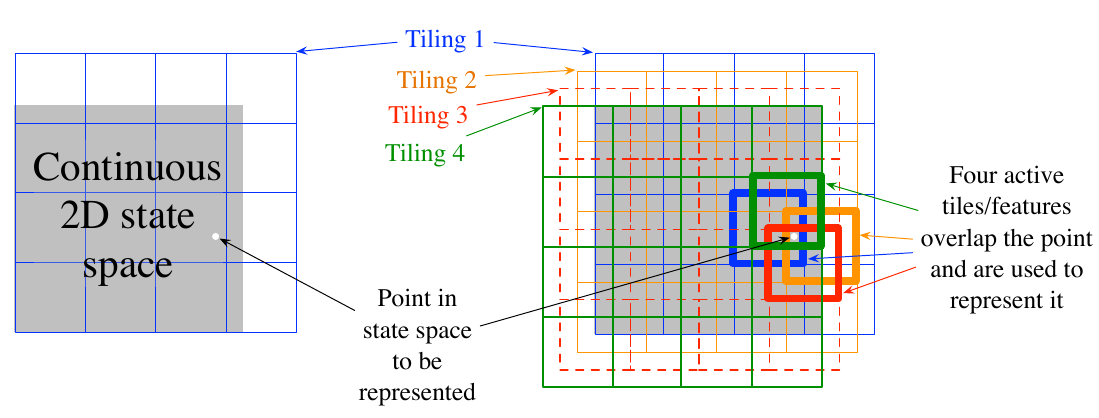
\includegraphics[width=1\linewidth]{c9-tile-coding.png}
  \caption{Multiple, overlapping grid-tilings on a limited 2D space. Thee tilings are offset from one another by a uniform amount in each dimension.}
  \label{fig:tile-coding}
\end{figure}

To get the strength of coarse coding, we need overlapping receptive fields. The advantages of tile coding
\begin{itemize}
\item the total active features at one time is the same for any state
\item computational advantages from its use of binary feature vectors (just sum all active features)
\item save memory
\end{itemize}

The choice of how to offset the tilings from each other affects generalization. Tile asymmetrical offsets are preferred. If the tilings are uniformly offset, then there are diagonal artifacts and substantial variations in the generalization, whereas with asymmetrically offset tilings the generalization is more spherical and homogeneous.

Extensive studies have been made of the effect of different displacement vectors on the generalization of tile coding.
In choosing a tiling strategy, one has to pick the number of the tilings and the shape of the tiles.

Another useful trick of reducing memory requirements is \textit{hashing} (Like one-to-many mapping).

\subsection{Selecting Step-Size Parameters Manually}

\subsection{Nonlinear Function Approximation: Artificial Neural Networks}

!! Note that neural network, like coarse coding/tile coding, is also a way of feature representation. State aggregation, coarse coding and tile coding are fixed representation. NN are flexible representation (due to learning)

This section is like a summary of the NN course. 

ANN is a network of interconnected units that have some of the properties of neurons.

A feedforward ANN has no loops in its network, i.e., there are no paths within the network by which a unit's output can influence its input. If an ANN has at least one loop in its connections, it is a recurrent rather than a feedforward ANN.

Hidden layers: layers that are neither input/output layers.

A real-valued weight is associated with each link.

The units in ANN are typically semi-linear units, meaning that they compute a weighted sum of their input signals and then apply to the result a nonlinear function (activation function). \textbf{Nonlinearity is essential}: if all the units have linear activation functions, the entire network is equivalent to a network without hidden layers (linear+linear = linear).

\textbf{Universal Approximation Property} An ANN with a single hidden layer containing a large enough finite number of sigmoid units can approximate any continuous function on a compact region of the network's input space to any degree of accuracy.

Training the hidden layers of an ANN is a way to auto create features appropriate for a given problem so that hierarchical representations can be produced w/o replying exclusively on hand-crafted features.

ANN typically learn by a stochastic gradient method. Each weight is adjusted in a direction aimed at improving the network's overall performance as measured by an objective function to be either min/maximized (that is, to estimate the partial derivative of an objective function w.r.t each weight, given the current values of all network's weights).

Backpropagation algorithm consists of alternating forward and backward passes through the network. (In later chapter, we discuss train ANN with RL instead of backpropagation).

Backpropagation may not work well for deep ANN. Because (1) the large number of weights can lead to overfitting; (2) the partial derivatives computed by its backward passes either decay rapidly (slow learning) or grow rapidly (unstable learning).

Overfitting is a problem for any function approximation method that adjusts functions with many degrees of freedom on the basis of limited training data.

Methods for reducing overfitting / improve training
\begin{itemize}
\item cross validation: stop training when performance begins to decrease on validation data different from the training data
\item regularization: modifying the objective function to discourage complexity of the approximation
\item weight sharing: introducing dependencies among the weights to reduce the number of degrees of freedom
\item dropout: during training, units are randomly removed from the network along with their connections
\item deep belief networks: deepest layers are trained first using unsupervised learning
\item batch normalization: normalizes the output of dep layers before they feed into the following layer
\item deep residual learning: sometimes it is easier to learn a function differs from the identify function than to learn the function itself (by adding shortcut, or skip connections)
\item deep convolution neural network
\end{itemize}

\paragraph{Compute the gradient of a single hidden layer neural network }

\begin{itemize}
\item step 1: define a loss on the parameters of the NN
\item step 2: find the parameters which minimize this loss function
\end{itemize}

Suppose we have input layer $\bm{s}$, hidden layer $\bm{x}$, output layer $\bm{y}$, input-hidden weight $\bm{A}$, hidden-output weight $\bm{B}$.

\begin{itemize}
\item $\bm{x} \doteq f_A(\bm{\psi})$, $\bm{\psi} \doteq \bm{s}\bm{A}$
\item $\bm{\hat{y}} \doteq f_B(\bm{\theta})$, $\bm{\theta} = \bm{x}\bm{B}$
\end{itemize}

Gradient w.r.t $\bm{B}$:
\begin{align*}
\frac{\partial L(\hat{\bm{y_k}}, \bm{y_k})}{\partial \bm{B_{jk}}} &= \frac{\partial L(\hat{\bm{y_k}}, \bm{y_k})}{\partial \hat{\bm{y_k}}}\frac{\partial \hat{\bm{y_k}}}{\partial \bm{B_{jk}}} \\
&= \frac{\partial L(\hat{\bm{y_k}}, \bm{y_k})}{\partial \hat{\bm{y_k}}}\frac{\partial f_{\bm{B}}(\theta_k)}{\partial\theta_k}\frac{\partial\theta_k}{\partial\bm{B}_{jk}} \\
&= \underbrace{\frac{\partial L(\hat{\bm{y_k}}, \bm{y_k})}{\partial \hat{\bm{y_k}}}\frac{\partial f_{\bm{B}}(\theta_k)}{\partial\theta_k}}_{\delta_k^{\bm{B}}} \bm{x_j}
\end{align*}

Note that the weight $\bm{A}$ also affect $\bm{x}$, so a chain rule set up is needed here. Gradient w.r.t $\bm{A}$:
\begin{align*}
\frac{\partial L(\hat{\bm{y_k}}, \bm{y_k})}{\partial \bm{A_{ij}}} &= \delta_k^{\bm{B}} \frac{\partial\theta_k}{\partial\bm{A}_{ij}} & \frac{\partial\theta_k}{\partial\bm{A}_{ij}} = \bm{B}_{jk}\frac{\partial \bm{x}_j}{\partial \bm{A}_{ij}} \\
&= \delta_k^{\bm{B}} \bm{B}_{jk}\frac{\partial \bm{x}_j}{\partial \bm{A}_{ij}} & \frac{\partial \bm{x}_j}{\partial \bm{A}_{ij}} = \frac{\partial f_{\bm{A}}(\psi_j) }{\partial \psi_j} \frac{\partial \psi_j}{\partial \bm{A}_{ij}} \\
&= \delta_k^{\bm{B}} \bm{B}_{jk} \frac{\partial f_{\bm{A}}(\psi_j) }{\partial \psi_j} \frac{\partial \psi_j}{\partial \bm{A}_{ij}} \\
&= \underbrace{\delta_k^{\bm{B}}\bm{B}_{jk} \frac{\partial f_{\bm{A}}(\psi_j) }{\partial \psi_j}}_{\delta_j^{\bm{A}}} \bm{s}_i
\end{align*}

Notice that both gradients can be rewritten in a similar form. They have a term $\delta$ that contains an error signal times their input.
$$\frac{\partial L(\hat{\bm{y_k}}, \bm{y_k})}{\partial \bm{A_{ij}}} = \delta_j^{\bm{A}}\bm{s}_i$$
$$\frac{\partial L(\hat{\bm{y_k}}, \bm{y_k})}{\partial \bm{B_{jk}}} = \delta_k^{\bm{B}}\bm{x_j}$$

\begin{tcolorbox}[width=1.1\textwidth,title={one-hidden layer backprop algorithm}]
for each i/o pair $(s,y)$ in dataset:

$\quad\delta_k^{\bm{B}} = \frac{\partial L(\hat{\bm{y_k}}, \bm{y_k})}{\partial \hat{\bm{y_k}}}\frac{\partial f_{\bm{B}}(\theta_k)}{\partial\theta_k}$

$\quad\nabla_{\bm{B}}^{jk}=\delta_k^{\bm{B}}\bm{x}_j$

$\quad\bm{B} = \bm{B} - \alpha_{\bm{B}}\nabla_{\bm{B}}$

$\quad\delta_j^{\bm{A}} = \delta_k^{\bm{B}}\bm{B}_{jk} \frac{\partial f_{\bm{A}}(\psi_j) }{\partial \psi_j}$

$\quad\nabla_j^{\bm{A}} = \delta_j^{\bm{A}}\bm{s}_i$

$\quad\bm{A} = \bm{A} - \alpha_{\bm{A}}\nabla_{\bm{A}}$
\end{tcolorbox}
First get prediction $\hat{y}$ (forward pass), then compute the gradients backwards from the output. Specifically, we first compute $\delta_{\bm{B}}$ and the gradient for B, then we use this gradient to update the parameters $\bm{B}$, the step size $\alpha_{\bm{B}}$. Next we update the parameters $\bm{A}$, we compute $\delta_{\bm{A}}$ which uses $\delta_{\bm{B}}$. Notice that by computing the gradients backwards, we avoid re-computing the same terms; In fact, this is the main idea behind backpropgation: it is simple GD with efficient strategy to compute gradients.

\subsection{Learning Objectives (UA RL MOOC)}

Lesson 1: Estimating Value Functions as Supervised Learning 

1. Understand how we can use parameterized functions to approximate value functions 

$\hat{v}(s, \bm{w})$

2. Explain the meaning of linear value function approximation 

$\hat{v}(s, \bm{w}) = \sum w_i x_i(s)$

3. Recognize that the tabular case is a special case of linear value function approximation. 

Consider each state has a corresponding vector (one-hot encoding)

4. Understand that there are many ways to parameterize an approximate value function 

ANN, decision tree etc

5. Understand what is meant by generalization and discrimination 

generalization: updates to the value estimate of one state influence the value of other states

discrimination:the ability to make the values for two states different to distinguish between the values for these two state.

6. Understand how generalization can be beneficial 

Generalization can speed up learning.

7. Explain why we want both generalization and discrimination from our function approximation 

Because we want generalization to speed up learning, and discrimination to distinguish really different states.

8. Understand how value estimation can be framed as a supervised learning problem 

Supervised learning involves approximating a function given a dataset of (input, target) pairs. For Monte-Carlo $(S_t, G_t)$. For TD $(S_t, R_t+\gamma\hat{v}(S_t, \bm{w}))$

9. Recognize not all function approximation methods are well suited for reinforcement learning 

Some are not suitable because they are designed for a fixed batch of data (offline learning, contrast to RL's online learning), or not designed for temporally correlated data (data in RL is always correlated).

Lesson 2: The Objective for On-policy Prediction 

10. Understand the mean-squared value error objective for policy evaluation 

We cannot guarantee perfect approximation for every state's value, so we need to define an objective, a measure of the distance between our approximation and the true values.
$$\overline{VE}(\bm{w}) \doteq \sum_{s\in\S} \underbrace{\mu(s)}_{\text{weight}} \underbrace{[v_\pi(s) - \hat{v}(s,\bm{w})]^2}_{\text{error}}$$

11. Explain the role of the state distribution in the objective 

$\mu(s)$ specifies how much we care for each state.
\begin{itemize}
\item It is a probability distribution
\item It has higher values for states that are visited more often
\item It serves as a weighting to minimize the error more in states that we care about
\end{itemize}

12. Understand the idea behind gradient descent and stochastic gradient descent 

We use SGD to optimize the objective $\overline{VE}$. (1) the gradient indicates the direction to increase/decrease the weight vectors; (2) the gradient gives the direction of steepest ascent

13. Outline the gradient Monte Carlo algorithm for value estimation 

see chap 9.3

14. Understand how state aggregation can be used to approximate the value function 

Group multiple states into one grouped state. One feature for each grouped state.

15. Apply Gradient Monte-Carlo with state aggregation 

see chap 9.3

Lesson 3: The Objective for TD 

16. Understand the TD-update for function approximation 

17. Highlight the advantages of TD compared to Monte-Carlo 

TD enables faster learning, continual and online learning; provides computational advantages

18. Outline the Semi-gradient TD(0) algorithm for value estimation 


see chap 9.3; semi-gradient TD as an approximation to SGD.

19. Understand that TD converges to a biased value estimate 

The TD target depends on our estimate of the value in the next state. This means our update could be biased because the estimate in our target may be inaccurate.

20. Understand that TD converges much faster than Gradient Monte Carlo 

TD can learn during the episode and has a lower variance update.

Lesson 4: Linear TD 

21. Derive the TD-update with linear function approximation 
$$\bm{w}_{t+1} = \bm{w} + \alpha[U_t - \hat{v}(S_t, \bm{w}_t)]\bm{x}(s)$$

22. Understand that tabular TD(0) is a special case of linear semi-gradient TD(0)

linear TD is a strict generalization on both tabular TD and TD with state aggregation. Recall the feature vector is like one-hot encoded vector, where the i-th=1, else 0 corresponds to i-th weight. 

23. Highlight the advantages of linear value function approximation over nonlinear 

\begin{itemize}
\item linear methods are simpler to understand and analyze mathematically
\item with good features, linear methods can learn quickly and achieve good prediction accuracy
\end{itemize}

linear semi-gradient TD (aka TD with linear function approximation)

-----------------------------------------

Lesson 1: Feature Construction for Linear Methods 

24. Describe the difference between coarse coding and tabular representations 

Tabular states can be represented with a binary one-hot encoding. Tabular representations become infeasible when state space is large (a state associate with a feature). We then introduced state aggregation to resolve this, where one feature represents many states.
Coarse coding is a further generalization of state aggregation, which allows overlapping of features (receptive fields).

25. Explain the trade-off when designing representations between discrimination and generalization 

The size, shape, and number of features (receptive fields) affect the generalization and discrimination, thus affecting learning accuracy.
For example, larger circle can generalize better, but discrimination is   worse.

26. Understand how different coarse coding schemes affect the functions that can be represented 

Recall the step-function approximation in the textbook.

27. Explain how tile coding is a (computationally?) convenient case of coarse coding 

Since grid is uniform, it's easy to compute which cell the current state is in.

28. Describe how designing the tilings affects the resultant representation 

The symmetry/asymmetry offsets affect tile coding's generalization and discrimination.

29. ...

Lesson 2: Neural Networks 

30. Define a neural network

\begin{itemize}
\item NN = input layer + hidden layer(s) + output layer
\item layer = node(s); layers are linked, each link is a real-valued weight
\item node contains non-linear function (active function)
\end{itemize}

31. Define activation functions

activation function = non-linear function (Sigmoid, ReLU, step function)

32. Define a feed-forward architecture 

A network without link from output to input.

33. Understand how neural networks are doing feature construction 

Tile coding has fixed parameters before learning, NN has both fixed and learned parameters. So NN can use both prior knowledge and knowledge from data to do feature construction.

34. Understand how neural networks are a non-linear function of state 

Non-linear activation function resulting in a non-linear function of the inputs.

35. Understand how deep networks are a composition of layers 

We can have many hidden layers (1) to allow composition of features. Composition can produce more specialized features by combining modular components; (2) to obtain abstractions, DNN compose many layers of lower-level of abstractions with each successive layer contributing to increasingly abstract representation.

36. Understand the trade-off between learning capacity and challenges presented by deeper networks 

Challenges mostly from overfitting and training efficiency.

Lesson 3: Training Neural Networks 

37. Understand the importance of initialization for neural networks 

If we choose a bad init parameters, we either have zero gradient or stuck in local optima.

38. Describe strategies for initializing neural networks 

\textbf{Method I}: randomly sample the initial weights from a normal distribution with small variance, and normalize the weights.
$$\bm{w}_{init}\sim \frac{N(0,1)}{\sqrt{n_{inputs}}}$$
This way, each neuron has a different output from other neurons within its layer. This provides a more diverse set of potential features. By keeping the variants small, we ensure that the output of each neuron is within the same range as its neighbors. By normalizing the weights, we prevent larger variance as number of neurons grows.

Adam Algorithm are Method II + Method III.
\textbf{Method II}: Update Momentum $M$
\begin{align*}
\bm{w}_{t+1} &\leftarrow \bm{w}_t - \alpha \nabla_{\bm{w}}L(\bm{w}_t)+\lambda M_t \\
M_{t+1} &\leftarrow \lambda M_t - \alpha \nabla_{\bm{w}}L
\end{align*}
The momentum term summarizes the history of the gradients using a decaying sum of gradients with decay rate $\lambda$. If recent updates in the same direction, then we have large momentum, making larger step; if recent updates in the opposite direction, then we kill the momentum.

\textbf{Method III}: vector step sizes

Instead of global step size, this uses different step sizes for different weights.

39. Describe optimization techniques for training neural networks

cross validation, regularization, dropout, residual learning etc

\end{document}